% Options for packages loaded elsewhere
\PassOptionsToPackage{unicode}{hyperref}
\PassOptionsToPackage{hyphens}{url}
%
\documentclass[
]{book}
\usepackage{lmodern}
\usepackage{amsmath}
\usepackage{ifxetex,ifluatex}
\ifnum 0\ifxetex 1\fi\ifluatex 1\fi=0 % if pdftex
  \usepackage[T1]{fontenc}
  \usepackage[utf8]{inputenc}
  \usepackage{textcomp} % provide euro and other symbols
  \usepackage{amssymb}
\else % if luatex or xetex
  \usepackage{unicode-math}
  \defaultfontfeatures{Scale=MatchLowercase}
  \defaultfontfeatures[\rmfamily]{Ligatures=TeX,Scale=1}
\fi
% Use upquote if available, for straight quotes in verbatim environments
\IfFileExists{upquote.sty}{\usepackage{upquote}}{}
\IfFileExists{microtype.sty}{% use microtype if available
  \usepackage[]{microtype}
  \UseMicrotypeSet[protrusion]{basicmath} % disable protrusion for tt fonts
}{}
\makeatletter
\@ifundefined{KOMAClassName}{% if non-KOMA class
  \IfFileExists{parskip.sty}{%
    \usepackage{parskip}
  }{% else
    \setlength{\parindent}{0pt}
    \setlength{\parskip}{6pt plus 2pt minus 1pt}}
}{% if KOMA class
  \KOMAoptions{parskip=half}}
\makeatother
\usepackage{xcolor}
\IfFileExists{xurl.sty}{\usepackage{xurl}}{} % add URL line breaks if available
\IfFileExists{bookmark.sty}{\usepackage{bookmark}}{\usepackage{hyperref}}
\hypersetup{
  pdftitle={CPS in Japan},
  pdfauthor={Keisuke Kawata},
  hidelinks,
  pdfcreator={LaTeX via pandoc}}
\urlstyle{same} % disable monospaced font for URLs
\usepackage{color}
\usepackage{fancyvrb}
\newcommand{\VerbBar}{|}
\newcommand{\VERB}{\Verb[commandchars=\\\{\}]}
\DefineVerbatimEnvironment{Highlighting}{Verbatim}{commandchars=\\\{\}}
% Add ',fontsize=\small' for more characters per line
\usepackage{framed}
\definecolor{shadecolor}{RGB}{248,248,248}
\newenvironment{Shaded}{\begin{snugshade}}{\end{snugshade}}
\newcommand{\AlertTok}[1]{\textcolor[rgb]{0.94,0.16,0.16}{#1}}
\newcommand{\AnnotationTok}[1]{\textcolor[rgb]{0.56,0.35,0.01}{\textbf{\textit{#1}}}}
\newcommand{\AttributeTok}[1]{\textcolor[rgb]{0.77,0.63,0.00}{#1}}
\newcommand{\BaseNTok}[1]{\textcolor[rgb]{0.00,0.00,0.81}{#1}}
\newcommand{\BuiltInTok}[1]{#1}
\newcommand{\CharTok}[1]{\textcolor[rgb]{0.31,0.60,0.02}{#1}}
\newcommand{\CommentTok}[1]{\textcolor[rgb]{0.56,0.35,0.01}{\textit{#1}}}
\newcommand{\CommentVarTok}[1]{\textcolor[rgb]{0.56,0.35,0.01}{\textbf{\textit{#1}}}}
\newcommand{\ConstantTok}[1]{\textcolor[rgb]{0.00,0.00,0.00}{#1}}
\newcommand{\ControlFlowTok}[1]{\textcolor[rgb]{0.13,0.29,0.53}{\textbf{#1}}}
\newcommand{\DataTypeTok}[1]{\textcolor[rgb]{0.13,0.29,0.53}{#1}}
\newcommand{\DecValTok}[1]{\textcolor[rgb]{0.00,0.00,0.81}{#1}}
\newcommand{\DocumentationTok}[1]{\textcolor[rgb]{0.56,0.35,0.01}{\textbf{\textit{#1}}}}
\newcommand{\ErrorTok}[1]{\textcolor[rgb]{0.64,0.00,0.00}{\textbf{#1}}}
\newcommand{\ExtensionTok}[1]{#1}
\newcommand{\FloatTok}[1]{\textcolor[rgb]{0.00,0.00,0.81}{#1}}
\newcommand{\FunctionTok}[1]{\textcolor[rgb]{0.00,0.00,0.00}{#1}}
\newcommand{\ImportTok}[1]{#1}
\newcommand{\InformationTok}[1]{\textcolor[rgb]{0.56,0.35,0.01}{\textbf{\textit{#1}}}}
\newcommand{\KeywordTok}[1]{\textcolor[rgb]{0.13,0.29,0.53}{\textbf{#1}}}
\newcommand{\NormalTok}[1]{#1}
\newcommand{\OperatorTok}[1]{\textcolor[rgb]{0.81,0.36,0.00}{\textbf{#1}}}
\newcommand{\OtherTok}[1]{\textcolor[rgb]{0.56,0.35,0.01}{#1}}
\newcommand{\PreprocessorTok}[1]{\textcolor[rgb]{0.56,0.35,0.01}{\textit{#1}}}
\newcommand{\RegionMarkerTok}[1]{#1}
\newcommand{\SpecialCharTok}[1]{\textcolor[rgb]{0.00,0.00,0.00}{#1}}
\newcommand{\SpecialStringTok}[1]{\textcolor[rgb]{0.31,0.60,0.02}{#1}}
\newcommand{\StringTok}[1]{\textcolor[rgb]{0.31,0.60,0.02}{#1}}
\newcommand{\VariableTok}[1]{\textcolor[rgb]{0.00,0.00,0.00}{#1}}
\newcommand{\VerbatimStringTok}[1]{\textcolor[rgb]{0.31,0.60,0.02}{#1}}
\newcommand{\WarningTok}[1]{\textcolor[rgb]{0.56,0.35,0.01}{\textbf{\textit{#1}}}}
\usepackage{longtable,booktabs}
\usepackage{calc} % for calculating minipage widths
% Correct order of tables after \paragraph or \subparagraph
\usepackage{etoolbox}
\makeatletter
\patchcmd\longtable{\par}{\if@noskipsec\mbox{}\fi\par}{}{}
\makeatother
% Allow footnotes in longtable head/foot
\IfFileExists{footnotehyper.sty}{\usepackage{footnotehyper}}{\usepackage{footnote}}
\makesavenoteenv{longtable}
\usepackage{graphicx}
\makeatletter
\def\maxwidth{\ifdim\Gin@nat@width>\linewidth\linewidth\else\Gin@nat@width\fi}
\def\maxheight{\ifdim\Gin@nat@height>\textheight\textheight\else\Gin@nat@height\fi}
\makeatother
% Scale images if necessary, so that they will not overflow the page
% margins by default, and it is still possible to overwrite the defaults
% using explicit options in \includegraphics[width, height, ...]{}
\setkeys{Gin}{width=\maxwidth,height=\maxheight,keepaspectratio}
% Set default figure placement to htbp
\makeatletter
\def\fps@figure{htbp}
\makeatother
\setlength{\emergencystretch}{3em} % prevent overfull lines
\providecommand{\tightlist}{%
  \setlength{\itemsep}{0pt}\setlength{\parskip}{0pt}}
\setcounter{secnumdepth}{5}
\usepackage{booktabs}
\ifluatex
  \usepackage{selnolig}  % disable illegal ligatures
\fi
\usepackage[]{natbib}
\bibliographystyle{apalike}

\title{CPS in Japan}
\author{Keisuke Kawata}
\date{2021-05-08}

\begin{document}
\maketitle

{
\setcounter{tocdepth}{1}
\tableofcontents
}
\hypertarget{summary}{%
\chapter{Summary}\label{summary}}

\begin{itemize}
\item
  Describe Japanese Labor market from 1986-2021.
\item
  Use the \href{https://www.stat.go.jp/english/data/roudou/index.html}{Labor force survey}, which is open-access and includes similar variables as the current population survey in U.S.
\end{itemize}

\hypertarget{simple-description-long-run}{%
\chapter{Simple description: Long-run}\label{simple-description-long-run}}

\hypertarget{environment}{%
\section{Environment}\label{environment}}

\begin{Shaded}
\begin{Highlighting}[]
\FunctionTok{library}\NormalTok{(data.table)}
\FunctionTok{library}\NormalTok{(tidytable)}
\FunctionTok{library}\NormalTok{(tidyverse)}
\FunctionTok{library}\NormalTok{(lubridate)}
\end{Highlighting}
\end{Shaded}

\hypertarget{data}{%
\section{Data}\label{data}}

\begin{Shaded}
\begin{Highlighting}[]
\NormalTok{raw }\OtherTok{\textless{}{-}} 
  \FunctionTok{fread}\NormalTok{(}\StringTok{"data/aggregate\_time\_series.csv"}\NormalTok{) }\SpecialCharTok{\%\textgreater{}\%}
  \FunctionTok{mutate}\NormalTok{(}\AttributeTok{date =} \FunctionTok{ymd}\NormalTok{(date),}
         \AttributeTok{employment =} \FunctionTok{as.numeric}\NormalTok{(就業者)}\SpecialCharTok{/}\FunctionTok{as.numeric}\NormalTok{(}\StringTok{\textasciigrave{}}\AttributeTok{15歳以上人口}\StringTok{\textasciigrave{}}\NormalTok{),}
         \AttributeTok{sex =} \FunctionTok{if\_else}\NormalTok{(性別 }\SpecialCharTok{==} \StringTok{"男"}\NormalTok{, }\StringTok{"male"}\NormalTok{, }\StringTok{"female"}\NormalTok{))}
\end{Highlighting}
\end{Shaded}

\hypertarget{employment-rate}{%
\section{Employment rate}\label{employment-rate}}

\begin{itemize}
\tightlist
\item
  Report \(e_{g,m,y} = \frac{Employment_{g,m,y}}{Population_{g,m,y}}\), where \(Employment_{g,m,y}\) and \(Population_{g,m,y}\) are numbers of employment and population over 15 years old in month \(m\), year \(y\) and gender group \(g\), respectively.
\end{itemize}

\begin{Shaded}
\begin{Highlighting}[]
\NormalTok{raw }\SpecialCharTok{\%\textgreater{}\%}
  \FunctionTok{ggplot}\NormalTok{(}\FunctionTok{aes}\NormalTok{(}\AttributeTok{x =}\NormalTok{ date,}
             \AttributeTok{y =}\NormalTok{ employment,}
             \AttributeTok{color =}\NormalTok{ sex)}
\NormalTok{         ) }\SpecialCharTok{+}
  \FunctionTok{geom\_line}\NormalTok{() }\SpecialCharTok{+}
  \FunctionTok{theme\_bw}\NormalTok{() }\SpecialCharTok{+}
  \FunctionTok{ylab}\NormalTok{(}\StringTok{"employment rate"}\NormalTok{)}
\end{Highlighting}
\end{Shaded}

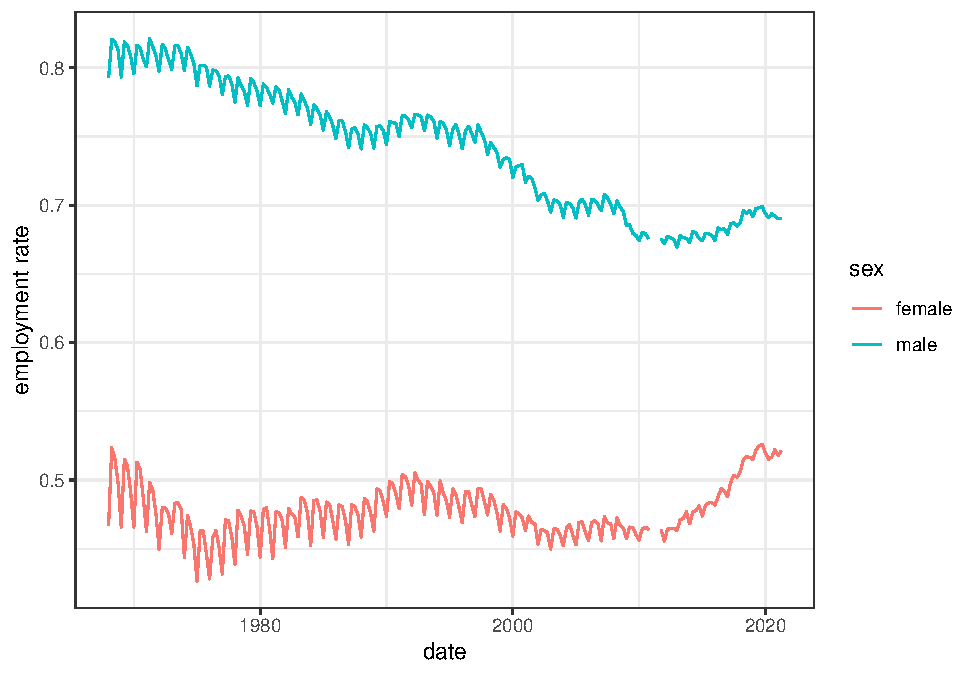
\includegraphics{CPS_Japan_files/figure-latex/unnamed-chunk-3-1.pdf}

\hypertarget{year-to-year-difference-of-employment-rate}{%
\section{Year-to-year difference of employment rate}\label{year-to-year-difference-of-employment-rate}}

\begin{itemize}
\tightlist
\item
  Report change of employment rate \(\tilde e_{g,m,y}=e_{g,m,y}-e_{g,m,y-1}\)
\end{itemize}

\begin{Shaded}
\begin{Highlighting}[]
\NormalTok{raw }\SpecialCharTok{\%\textgreater{}\%}
  \FunctionTok{mutate}\NormalTok{(}\AttributeTok{year =} \FunctionTok{year}\NormalTok{(date),}
         \AttributeTok{month =} \FunctionTok{month}\NormalTok{(date)}
\NormalTok{         ) }\SpecialCharTok{\%\textgreater{}\%}
  \FunctionTok{arrange}\NormalTok{(sex,}
\NormalTok{          month,}
\NormalTok{          year) }\SpecialCharTok{\%\textgreater{}\%}
  \FunctionTok{group\_by}\NormalTok{(sex,}
\NormalTok{           month) }\SpecialCharTok{\%\textgreater{}\%}
  \FunctionTok{mutate}\NormalTok{(}\AttributeTok{employment =}\NormalTok{ employment }\SpecialCharTok{{-}} \FunctionTok{lag}\NormalTok{(employment)) }\SpecialCharTok{\%\textgreater{}\%}
\NormalTok{  ungroup }\SpecialCharTok{\%\textgreater{}\%}
  \FunctionTok{filter}\NormalTok{(year }\SpecialCharTok{\textgreater{}=} \DecValTok{1969}\NormalTok{) }\SpecialCharTok{\%\textgreater{}\%}
  \FunctionTok{ggplot}\NormalTok{(}\FunctionTok{aes}\NormalTok{(}\AttributeTok{x =}\NormalTok{ date,}
             \AttributeTok{y =}\NormalTok{ employment,}
             \AttributeTok{color =}\NormalTok{ sex)}
\NormalTok{         ) }\SpecialCharTok{+}
  \FunctionTok{geom\_line}\NormalTok{() }\SpecialCharTok{+}
  \FunctionTok{geom\_hline}\NormalTok{(}\AttributeTok{yintercept =} \DecValTok{0}\NormalTok{) }\SpecialCharTok{+}
  \FunctionTok{ylab}\NormalTok{(}\StringTok{""}\NormalTok{) }\SpecialCharTok{+}
  \FunctionTok{xlab}\NormalTok{(}\StringTok{""}\NormalTok{) }\SpecialCharTok{+}
  \FunctionTok{theme\_bw}\NormalTok{() }\SpecialCharTok{+}
  \FunctionTok{theme}\NormalTok{(}\AttributeTok{legend.position =} \StringTok{"bottom"}\NormalTok{)}
\end{Highlighting}
\end{Shaded}

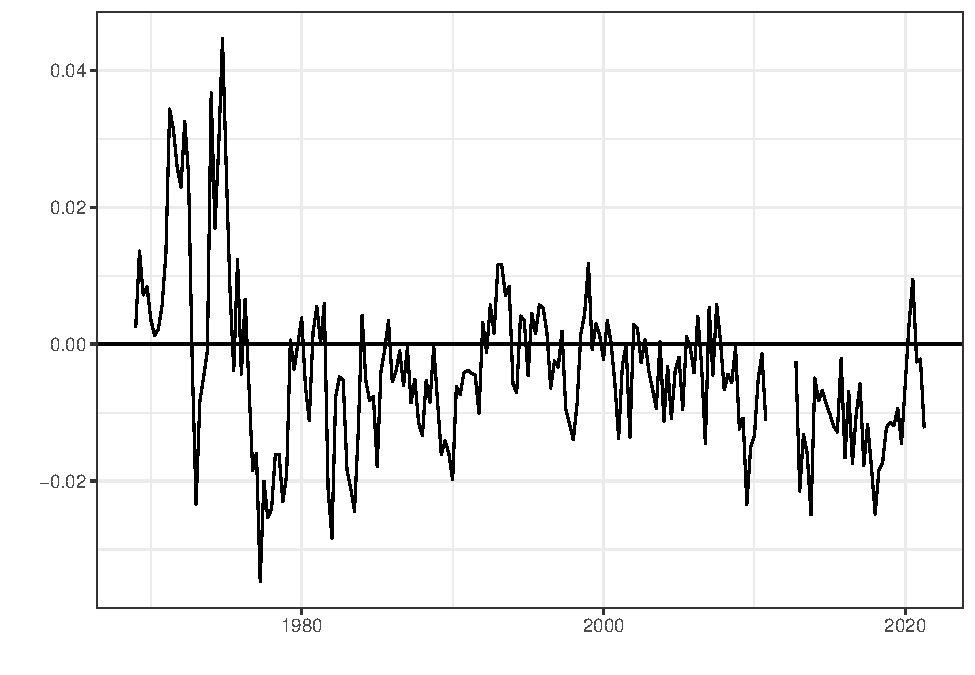
\includegraphics{CPS_Japan_files/figure-latex/unnamed-chunk-4-1.pdf}

\hypertarget{gender-gap}{%
\section{Gender gap}\label{gender-gap}}

\begin{itemize}
\tightlist
\item
  Report change of employment rate \(\tilde e_{male,m,y} - \tilde e_{female,m,y}\)
\end{itemize}

\begin{Shaded}
\begin{Highlighting}[]
\NormalTok{raw }\SpecialCharTok{\%\textgreater{}\%}
  \FunctionTok{mutate}\NormalTok{(}\AttributeTok{year =} \FunctionTok{year}\NormalTok{(date),}
         \AttributeTok{month =} \FunctionTok{month}\NormalTok{(date)}
\NormalTok{         ) }\SpecialCharTok{\%\textgreater{}\%}
  \FunctionTok{arrange}\NormalTok{(sex,}
\NormalTok{          month,}
\NormalTok{          year) }\SpecialCharTok{\%\textgreater{}\%}
  \FunctionTok{group\_by}\NormalTok{(sex,}
\NormalTok{           month) }\SpecialCharTok{\%\textgreater{}\%}
  \FunctionTok{mutate}\NormalTok{(}\AttributeTok{employment =}\NormalTok{ employment }\SpecialCharTok{{-}} \FunctionTok{lag}\NormalTok{(employment)) }\SpecialCharTok{\%\textgreater{}\%}
\NormalTok{  ungroup }\SpecialCharTok{\%\textgreater{}\%}
  \FunctionTok{filter}\NormalTok{(year }\SpecialCharTok{\textgreater{}=} \DecValTok{1969}\NormalTok{) }\SpecialCharTok{\%\textgreater{}\%}
  \FunctionTok{arrange}\NormalTok{(date,}
\NormalTok{          sex) }\SpecialCharTok{\%\textgreater{}\%}
  \FunctionTok{group\_by}\NormalTok{(date) }\SpecialCharTok{\%\textgreater{}\%}
  \FunctionTok{mutate}\NormalTok{(}\AttributeTok{employment =}\NormalTok{ employment }\SpecialCharTok{{-}} \FunctionTok{lag}\NormalTok{(employment)) }\SpecialCharTok{\%\textgreater{}\%}
\NormalTok{  ungroup }\SpecialCharTok{\%\textgreater{}\%}
  \FunctionTok{filter}\NormalTok{(sex }\SpecialCharTok{==} \StringTok{"male"}\NormalTok{) }\SpecialCharTok{\%\textgreater{}\%}
  \FunctionTok{ggplot}\NormalTok{(}\FunctionTok{aes}\NormalTok{(}\AttributeTok{x =}\NormalTok{ date,}
             \AttributeTok{y =}\NormalTok{ employment)}
\NormalTok{         ) }\SpecialCharTok{+}
  \FunctionTok{geom\_line}\NormalTok{() }\SpecialCharTok{+}
  \FunctionTok{geom\_hline}\NormalTok{(}\AttributeTok{yintercept =} \DecValTok{0}\NormalTok{) }\SpecialCharTok{+}
  \FunctionTok{ylab}\NormalTok{(}\StringTok{""}\NormalTok{) }\SpecialCharTok{+}
  \FunctionTok{xlab}\NormalTok{(}\StringTok{""}\NormalTok{) }\SpecialCharTok{+}
  \FunctionTok{theme\_bw}\NormalTok{()}
\end{Highlighting}
\end{Shaded}

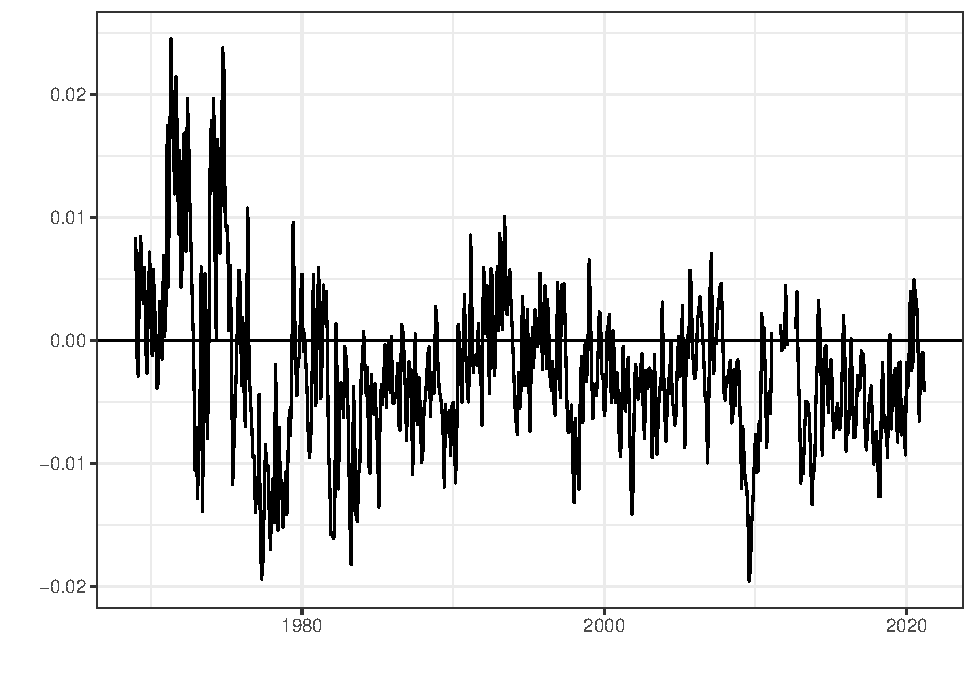
\includegraphics{CPS_Japan_files/figure-latex/unnamed-chunk-5-1.pdf}

\hypertarget{simple-description}{%
\chapter{Simple description}\label{simple-description}}

\hypertarget{environment-1}{%
\section{Environment}\label{environment-1}}

\begin{Shaded}
\begin{Highlighting}[]
\FunctionTok{library}\NormalTok{(data.table)}
\FunctionTok{library}\NormalTok{(tidytable)}
\FunctionTok{library}\NormalTok{(tidyverse)}
\FunctionTok{library}\NormalTok{(lubridate)}
\end{Highlighting}
\end{Shaded}

\hypertarget{data-1}{%
\section{Data}\label{data-1}}

\begin{Shaded}
\begin{Highlighting}[]
\NormalTok{raw }\OtherTok{\textless{}{-}} 
  \FunctionTok{fread}\NormalTok{(}\StringTok{"data/aggregate\_time\_series.csv"}\NormalTok{) }\SpecialCharTok{\%\textgreater{}\%}
  \FunctionTok{mutate}\NormalTok{(}\AttributeTok{date =} \FunctionTok{ymd}\NormalTok{(date),}
         \AttributeTok{employment =} \FunctionTok{as.numeric}\NormalTok{(就業者)}\SpecialCharTok{/}\FunctionTok{as.numeric}\NormalTok{(}\StringTok{\textasciigrave{}}\AttributeTok{15歳以上人口}\StringTok{\textasciigrave{}}\NormalTok{),}
         \AttributeTok{sex =} \FunctionTok{if\_else}\NormalTok{(性別 }\SpecialCharTok{==} \StringTok{"男"}\NormalTok{, }\StringTok{"male"}\NormalTok{, }\StringTok{"female"}\NormalTok{))}
\end{Highlighting}
\end{Shaded}

\hypertarget{employment-rate-1}{%
\section{Employment rate}\label{employment-rate-1}}

\begin{itemize}
\tightlist
\item
  Report \(e_{g,m,y} = \frac{Employment_{g,m,y}}{Population_{g,m,y}}\), where \(Employment_{g,m,y}\) and \(Population_{g,m,y}\) are numbers of employment and population over 15 years old in month \(m\), year \(y\) and gender group \(g\), respectively.
\end{itemize}

\begin{Shaded}
\begin{Highlighting}[]
\NormalTok{raw }\SpecialCharTok{\%\textgreater{}\%}
  \FunctionTok{filter}\NormalTok{(date }\SpecialCharTok{\textgreater{}=} \StringTok{"2019{-}01{-}01"}\NormalTok{) }\SpecialCharTok{\%\textgreater{}\%}
  \FunctionTok{ggplot}\NormalTok{(}\FunctionTok{aes}\NormalTok{(}\AttributeTok{x =}\NormalTok{ date,}
             \AttributeTok{y =}\NormalTok{ employment,}
             \AttributeTok{color =}\NormalTok{ sex)}
\NormalTok{         ) }\SpecialCharTok{+}
  \FunctionTok{geom\_line}\NormalTok{() }\SpecialCharTok{+}
  \FunctionTok{theme\_bw}\NormalTok{() }\SpecialCharTok{+}
  \FunctionTok{ylab}\NormalTok{(}\StringTok{"employment rate"}\NormalTok{)}
\end{Highlighting}
\end{Shaded}

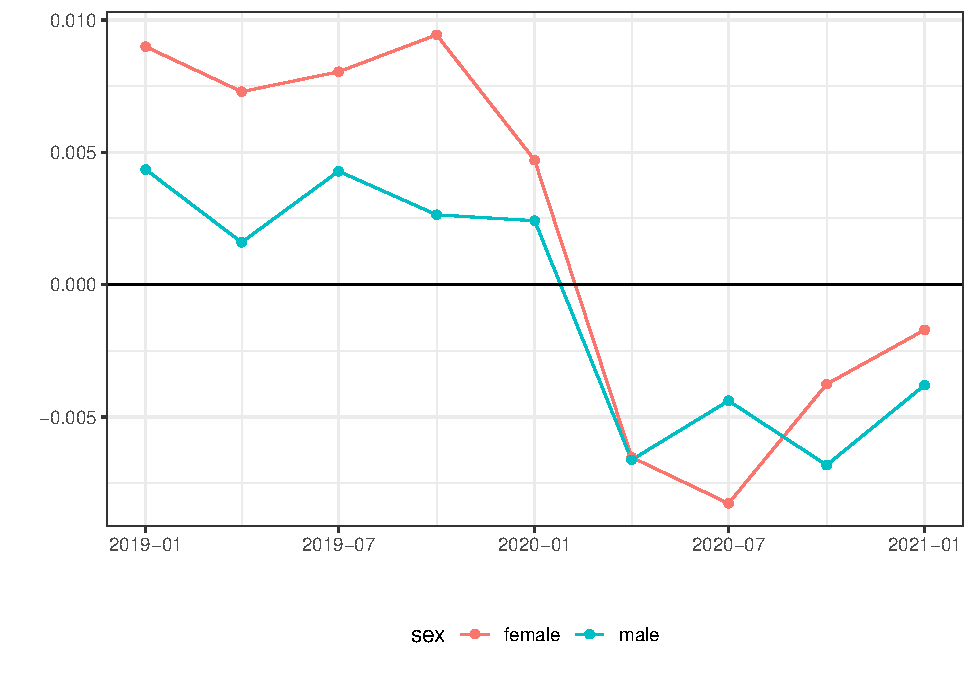
\includegraphics{CPS_Japan_files/figure-latex/unnamed-chunk-8-1.pdf}

\hypertarget{year-to-year-difference-of-employment-rate-1}{%
\section{Year-to-year difference of employment rate}\label{year-to-year-difference-of-employment-rate-1}}

\begin{itemize}
\tightlist
\item
  Report change of employment rate \(\tilde e_{g,m,y}=e_{g,m,y}-e_{g,m,y-1}\)
\end{itemize}

\begin{Shaded}
\begin{Highlighting}[]
\NormalTok{raw }\SpecialCharTok{\%\textgreater{}\%}
  \FunctionTok{mutate}\NormalTok{(}\AttributeTok{year =} \FunctionTok{year}\NormalTok{(date),}
         \AttributeTok{month =} \FunctionTok{month}\NormalTok{(date)}
\NormalTok{         ) }\SpecialCharTok{\%\textgreater{}\%}
  \FunctionTok{arrange}\NormalTok{(sex,}
\NormalTok{          month,}
\NormalTok{          year) }\SpecialCharTok{\%\textgreater{}\%}
  \FunctionTok{group\_by}\NormalTok{(sex,}
\NormalTok{           month) }\SpecialCharTok{\%\textgreater{}\%}
  \FunctionTok{mutate}\NormalTok{(}\AttributeTok{employment =}\NormalTok{ employment }\SpecialCharTok{{-}} \FunctionTok{lag}\NormalTok{(employment)) }\SpecialCharTok{\%\textgreater{}\%}
\NormalTok{  ungroup }\SpecialCharTok{\%\textgreater{}\%}
  \FunctionTok{filter}\NormalTok{(year }\SpecialCharTok{\textgreater{}=} \DecValTok{2019}\NormalTok{) }\SpecialCharTok{\%\textgreater{}\%}
  \FunctionTok{ggplot}\NormalTok{(}\FunctionTok{aes}\NormalTok{(}\AttributeTok{x =}\NormalTok{ date,}
             \AttributeTok{y =}\NormalTok{ employment,}
             \AttributeTok{color =}\NormalTok{ sex)}
\NormalTok{         ) }\SpecialCharTok{+}
  \FunctionTok{geom\_line}\NormalTok{() }\SpecialCharTok{+}
  \FunctionTok{geom\_point}\NormalTok{() }\SpecialCharTok{+}
  \FunctionTok{geom\_hline}\NormalTok{(}\AttributeTok{yintercept =} \DecValTok{0}\NormalTok{) }\SpecialCharTok{+}
  \FunctionTok{ylab}\NormalTok{(}\StringTok{""}\NormalTok{) }\SpecialCharTok{+}
  \FunctionTok{xlab}\NormalTok{(}\StringTok{""}\NormalTok{) }\SpecialCharTok{+}
  \FunctionTok{theme\_bw}\NormalTok{() }\SpecialCharTok{+}
  \FunctionTok{theme}\NormalTok{(}\AttributeTok{legend.position =} \StringTok{"bottom"}\NormalTok{)}
\end{Highlighting}
\end{Shaded}

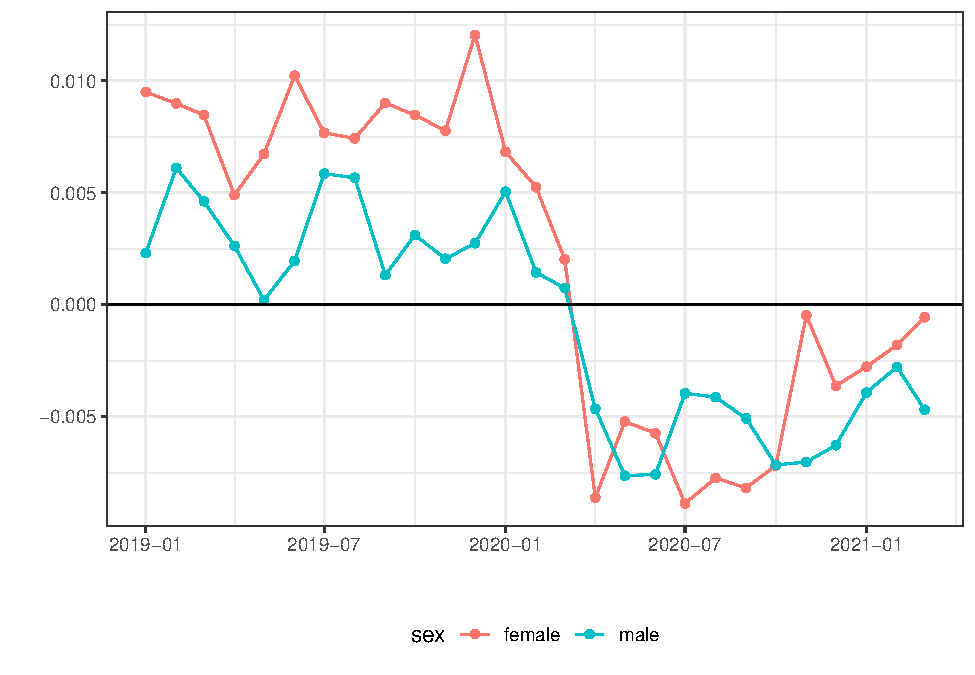
\includegraphics{CPS_Japan_files/figure-latex/unnamed-chunk-9-1.pdf}

\hypertarget{gender-gap-1}{%
\section{Gender gap}\label{gender-gap-1}}

\begin{itemize}
\tightlist
\item
  Report change of employment rate \(\tilde e_{male,m,y} - \tilde e_{female,m,y}\)
\end{itemize}

\begin{Shaded}
\begin{Highlighting}[]
\NormalTok{raw }\SpecialCharTok{\%\textgreater{}\%}
  \FunctionTok{mutate}\NormalTok{(}\AttributeTok{year =} \FunctionTok{year}\NormalTok{(date),}
         \AttributeTok{month =} \FunctionTok{month}\NormalTok{(date)}
\NormalTok{         ) }\SpecialCharTok{\%\textgreater{}\%}
  \FunctionTok{arrange}\NormalTok{(sex,}
\NormalTok{          month,}
\NormalTok{          year) }\SpecialCharTok{\%\textgreater{}\%}
  \FunctionTok{group\_by}\NormalTok{(sex,}
\NormalTok{           month) }\SpecialCharTok{\%\textgreater{}\%}
  \FunctionTok{mutate}\NormalTok{(}\AttributeTok{employment =}\NormalTok{ employment }\SpecialCharTok{{-}} \FunctionTok{lag}\NormalTok{(employment)) }\SpecialCharTok{\%\textgreater{}\%}
\NormalTok{  ungroup }\SpecialCharTok{\%\textgreater{}\%}
  \FunctionTok{filter}\NormalTok{(year }\SpecialCharTok{\textgreater{}=} \DecValTok{2019}\NormalTok{) }\SpecialCharTok{\%\textgreater{}\%}
  \FunctionTok{arrange}\NormalTok{(date,}
\NormalTok{          sex) }\SpecialCharTok{\%\textgreater{}\%}
  \FunctionTok{group\_by}\NormalTok{(date) }\SpecialCharTok{\%\textgreater{}\%}
  \FunctionTok{mutate}\NormalTok{(}\AttributeTok{employment =}\NormalTok{ employment }\SpecialCharTok{{-}} \FunctionTok{lag}\NormalTok{(employment)) }\SpecialCharTok{\%\textgreater{}\%}
\NormalTok{  ungroup }\SpecialCharTok{\%\textgreater{}\%}
  \FunctionTok{filter}\NormalTok{(sex }\SpecialCharTok{==} \StringTok{"male"}\NormalTok{) }\SpecialCharTok{\%\textgreater{}\%}
  \FunctionTok{ggplot}\NormalTok{(}\FunctionTok{aes}\NormalTok{(}\AttributeTok{x =}\NormalTok{ date,}
             \AttributeTok{y =}\NormalTok{ employment)}
\NormalTok{         ) }\SpecialCharTok{+}
  \FunctionTok{geom\_line}\NormalTok{() }\SpecialCharTok{+}
  \FunctionTok{geom\_point}\NormalTok{() }\SpecialCharTok{+}
  \FunctionTok{geom\_hline}\NormalTok{(}\AttributeTok{yintercept =} \DecValTok{0}\NormalTok{) }\SpecialCharTok{+}
  \FunctionTok{ylab}\NormalTok{(}\StringTok{""}\NormalTok{) }\SpecialCharTok{+}
  \FunctionTok{xlab}\NormalTok{(}\StringTok{""}\NormalTok{) }\SpecialCharTok{+}
  \FunctionTok{theme\_bw}\NormalTok{()}
\end{Highlighting}
\end{Shaded}

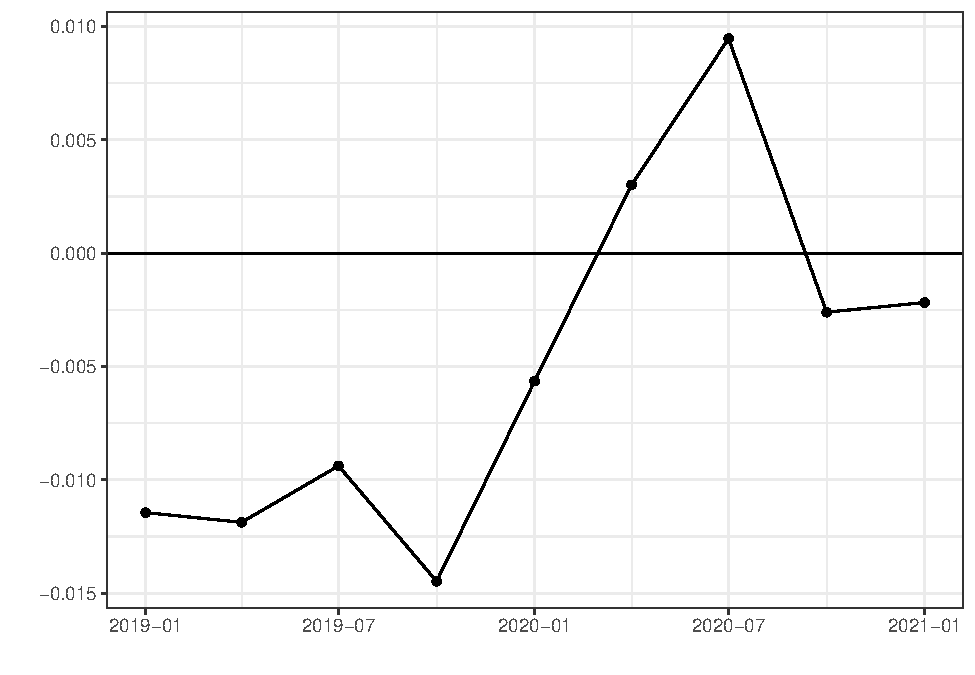
\includegraphics{CPS_Japan_files/figure-latex/unnamed-chunk-10-1.pdf}

  \bibliography{book.bib,packages.bib}

\end{document}
